\chapter{Seasons and Calendars across cultures}
\label{ch:seasons}

This chapter focusses on the qualitative research component.
It discusses interview methods, considerations for indigenous knowledge, and integration with literature.
The primary results are a reflection on process and outcomes, and a Yolngu calendar.


\section{Methods}

I initially planned to gather qualitative data on the Yolngu seasonal calendar
from published resources and interviews with Yolngu people.
Over the course of my research, several unforseen approaches have also proved important.

I conducted a series of informal, semistructured interviews centered around discussion of seasons and climate.
Recruitment was primarily by a `snowball' pattern, where participants were asked to
suggest further potential participants.
See \autoref{sec:ethics} for details of the human ethics approval.
The main `seeds' of this pattern were personal contacts, some Yolngu and some non-indigenous
people who have spent decades living and working in remote communities.
I followed several disconnected threads such as the \citet{CSIROcals} project,
which helped to clarify and test my interpretation of the interviews.

I rely on four sources of qualitative knowledge and context for the Yolngu seasons, in rough order of importance:

\begin{itemize}
\item Interview with Yolngu people form the basis of my qualitative research, and
        are the definitive source of information about Yolngu seasons.
\item Interviews and discussion with non-indigenous researchers or teachers experienced
        in remote communities help contextualise this knowledge, and warned of
        common misinterpretations - as well as pointing out nuance.
\item Published literature, particularly around cross-cultural research \citep[eg.][]{smith1999},
        Australian indigenous seasons \citep[eg.][]{prober2011,oconnor2010}, and Yolngu
        seasons directly \citep{davis1989}.
\item Grey literature, such as posters produced for use in remote schools, workbooks
        for cross-cultural teacher training, etc.
\end{itemize}

Semi-structured interviews with Yolngu participants are my primary source of information and indispensible.
They tended to alternate between rambling discussions of seasons and calendars,
and focussed lessons on particular aspects of the seasons.

The literature contextualises and informs the interviews, and suggested many fruitful
directions for direct questions or later searches for documents.

Following the interviews, I also engaged in substantial reflection on the nature of
my questions and the ambiguity of the responses and data I collected.



\section{Results and Discussion}

The qualitative results are fall into four subsections.
First, a review of the literature relevant to Yolngu seasons, including unpublished documents.
Second, personal reflections following my interviews, as above.
Third, a summary of the emergent themes in my interviews.
Fourth and finally, a Yolngu seasonal calendar drawn from interiew responses and aligned with \citet{davis1989}.


\subsection{Literature describing Yolngu Seasons}
This section is focussed on \textit{Man of All Seasons} \citep{davis1989},
with extra commentary from various posters supplied by Ian Morris.


\subsection{Reflection - Complex Calendars as an emergent theme}

`Calendar' and `season' are not concepts that translate directly across cultures. 

Discuss how I realised this, by re-listening to recordings, and that I was expecting something unforeseen (but not like this!).  

\emph{TODO: expand points to paragraphs, with quotes}

\begin{itemize}
\item all in english
\item what is a season
\item what is a calendar
\item there is no ``the'' yolngu calendar - varies spatially,
        multiple seasonal calendars for different temporal scales with varied purposes
\item `simple fact-finding' really isn't!
\end{itemize}



\subsection{Yolngu Seasons - varying by location and temporal scale}

Yolngu participants discussed three levels of seasons:
\begin{itemize}
\item A Wet-Dry seasonality, based on the monsoon winds;
\item A six-season calendar defined primarily by wind, rain, and temperature; and
\item Phenological seasons, where ecological events signal appropriate activities.
\end{itemize}

A similar system is visible in \autoref{fig:tiwi-seasons}, showing the Tiwi seaons at
a monsoonal level, as well as more precise seasons defined by weather or ecology.


\begin{landscape}
\begin{figure}[p]
    \centering
    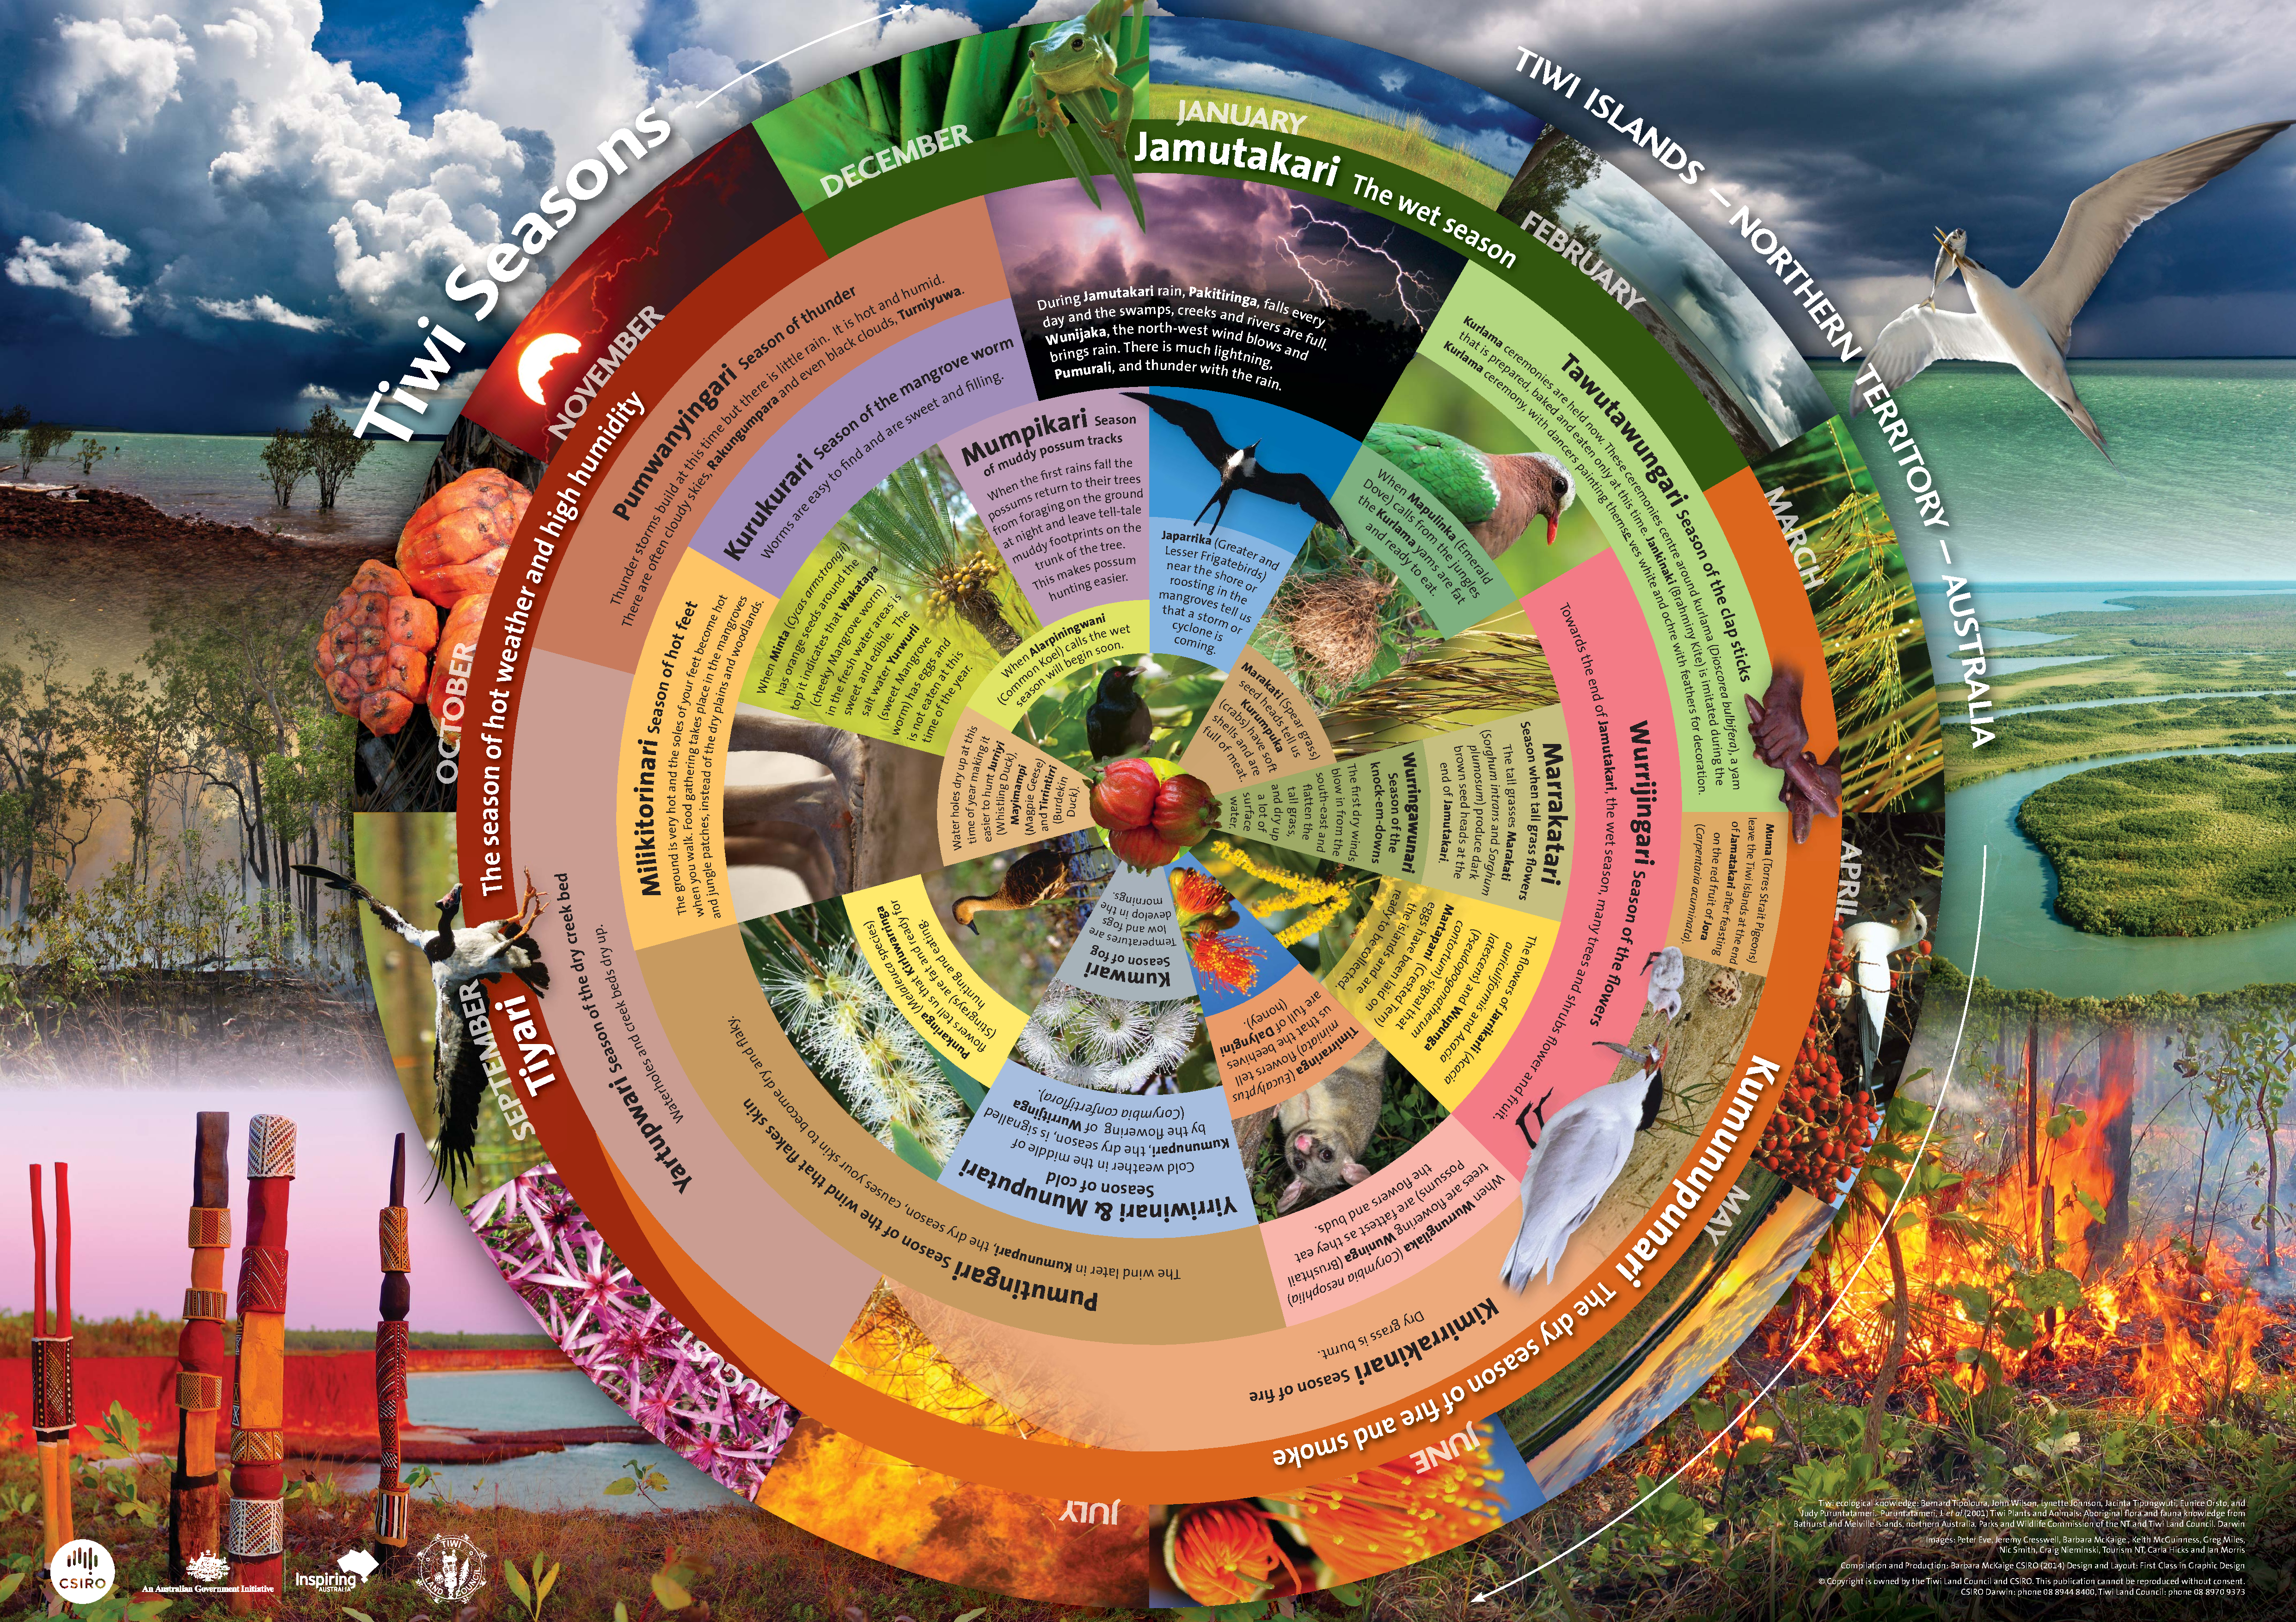
\includegraphics[width=\paperwidth]{TiwiSeasons.pdf}
    \caption[The Tiwi Seasons Calendar by \citet{CSIROcals}]{
        The Tiwi Seasons Calendar by \citet{CSIROcals}.
        This calendar shows month of year in the outermost ring,
        then three `major' Tiwi seasons recognised by weather.
        Note that \textit{Kumunupunari} does not have a sharp boundary with \textit{Tiyari}!
        Within this ring are smaller seasons, recognised by weather
        or ecological events and associated with particular activities.
        This format is designed for the circle to rotate, encouraging interaction or observation.
        }
    \label{fig:tiwi-seasons}
\end{figure}
\end{landscape}


Of the three levels of seasons recognised by Yolngu,
the wet/dry monsoon seasonal cycle is most likely familiar to non-indigenous people -
especially in the tropics.  Yolngu participants emphasised that these seasons
are \emph{not} recognised by rainfall, but rather the direction of prevailing winds.

ADD QUOTE HERE

Interestingly, this mirrors the meteorological definition of monsoon, where rainfall is less important than
the location of the intertropical convergence zone and consequent direction of prevailing wind.
This shared understanding of monsoon seasonality should not go unremarked -
but does direct this research to the more local seasonal patterns.


The phenological seasons are very interesting, but several practical barriers to detailed study exist.
For this thesis, the paucity of relevant phenological data means that
investigating these seasons is beyond scope.
Further research would require living in the study area for several years,
and the results are not generalisable as calendars with these timescales and indicators
vary between communities even in the same language group.  INSERT SUPPORTING QUOTES


Lorem Ipsum six seasons, using because, details in next subsection.  ADD DETAILS



\subsection{Describing a Yolnu Seasonal Calendar}

The remainder of this thesis focusses on a particular Yolnu calendar,
that of six seasons as recognised at Galiwinku on Elcho Island.
See \autoref{fig:yolngu-seasons} for a graphical representation of these seasons.

The descriptions below are drawn from interviews with participants from Galiwinku.
I also present selected quotations from \textit{Man of All Seasons} \citep{davis1989},
which describe the seasons as experienced at Milingimbi.
Note that weather data for both is analysed in \autoref{ch:quantify},
including observations on differences in seasonality.


\paragraph{Dhuludur} marks the beginning of the seasonal cycle.

\citet{davis1989} calls Dhuludur the `pre-wet' season:
\blockquote{
    The weather is cool and still during the night, with mists settling in the night and rising in the morning after a light northwest wind during the day. ...
    The winds are mixed up, with southwest, southeast, northeast, and northwest winds each blowing at different times, often during the same day. ...
    The weather begins to get hot and humid as the clouds build up more and more each day.
    When the sky is covered by heavy cloud, the `female' thunder brings the first rain [often from the southeast].
    After the first rain, other winds bring heavy rain. ...
    
    Towards the end of the pre-wet season the rain is being brought only by the northwest wind.
    It rains almost every evening.
    This is the start of the next season, which is signified by heavy rains and growth.
}

The sea is calm and the skies are clear.


\paragraph{Barramirri}

\citet{davis1989} calls Barramirri `the season of heavy rain and growth':
\blockquote{
    The heavy rain is brought by the northwest wind. It comes every day, indicating that the seasons have changed. ...
    As the northwest wind brings daily storms, the sea is dirty and rough. ...
    The inundation is so extensive that much of the inland is now one continious sheet of water [, which will not drain until the end of the wet season]. ...
    
    Many plants flower, an the rain becomes infrequent and sometimes stops for several weeks.
    These are indications that the season of heavy rain is drawing to a close.
}


\paragraph{Mayaltha} is the season of plenty - at Galiwinku.  

QUOTE R on whatever tye of food, how to recognise season.

\citet{davis1989} calls Mayaltha the `flowering' season:
\blockquote{
    [The Flowering Season] is marked by an abundance of plants that flower, bright sunny days, cool breezes, and occasional rain. ...
    
    During the early wet season strong winds often brought the rain.
    The wind then stopped as the rain fell.
    Now the winds blow hard even when it is raining.
    The rains do not come daily any more, but only every week or two.
}


\paragraph{Midawarr} is recognised at Milingimbi as the season of plenty, but folded into Mayaltha at Galiwinku.

Some participants did not name this as a separate season.
It is instead seen as part of Mayaltha, which becomes a major season - along with wet and dry.
This is a concrete example of the variation in calendars between communities and the complexity of seasons over different timescales,
making them a rich source of ecological knowledge and a frustrating subject of study!

\citet{davis1989} calls Midawarr the `fruiting' season:
\blockquote{
    The east wind signals the beginning of the time of abundant food ... the first southeast wind blows gently in the early morning. ...
    
    The daily storms and strong winds are nearly over.  The northwest wind changes to the northeast, bring rough seas.
    Early in the season the storms still bring heavy rain daily.
    
    By the middle of the season the wind has changed to he east and heavy storms are less frequent.
    Light easterly winds blow throughout most of the day bringing cooler weather. ...
    
    Shortly after sunrise the east wind blows and continues for the rest of the day.
    
    Towards the end of the fruiting season, the days are becoming more like the early dry season with morning mists.
    One last storm of the wet season comes and flattens [tall dry grass].\footnote{SUch storms are widely known as `knock-em-downs'}
    This storm is brought by strong southeast wind, which is the main dry season wind.
}


\paragraph{Dharrathamirri}

\citet{davis1989} calls Dharrathamirri the `early dry' season:
\blockquote{
    The nights are cool and these is mist early on some mornings.
    The southeast wind swings further south, to become the south-southeast wind called the trade wind. ...
    
    XXXX FILL OUT from p53
    
    Note stellar indicators - Orion setting early
}


\paragraph{Rarrandharr}

\citet{davis1989} calls Rarrandharr the `main dry' season:
\blockquote{
    The east-southeast wind blows; the cold mornings and mist are nearly gone.
    This is an intermediate season between the early dry and main dry seasons.
    It is very short, lasting only a few weeks.
    
    The warmer southeast wind starts to blow...
    When the wind dies down, soon the three stars of \textit{Djulpan} (Orion's Belt) will begin to rise in the east before people go to sleep at night.
    
    When the mangoes are nearly finished, the dry season is also near its end.
    The weather changes and thunder begins.
}








